  
  
  \tikzset{every picture/.style={line width=0.75pt}} %set default line width to 0.75pt        
  
  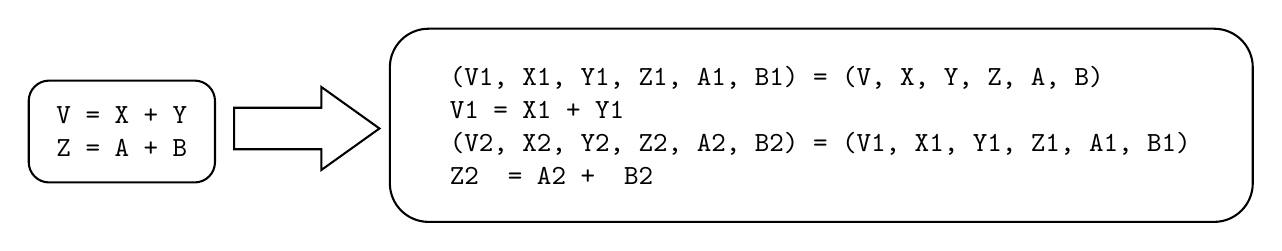
\begin{tikzpicture}[x=0.75pt,y=0.75pt,yscale=-1,xscale=1]
  %uncomment if require: \path (0,300); %set diagram left start at 0, and has height of 300
  
  %Rounded Rect [id:dp257541138848127] 
  \draw   (7,42.75) .. controls (7,37.33) and (11.39,32.93) .. (16.81,32.93) -- (86.94,32.93) .. controls (92.36,32.93) and (96.75,37.33) .. (96.75,42.75) -- (96.75,72.19) .. controls (96.75,77.61) and (92.36,82) .. (86.94,82) -- (16.81,82) .. controls (11.39,82) and (7,77.61) .. (7,72.19) -- cycle ;
  %Right Arrow [id:dp5774776776599181] 
  \draw   (106,46) -- (148,46) -- (148,36) -- (176,56) -- (148,76) -- (148,66) -- (106,66) -- cycle ;
  %Rounded Rect [id:dp9338900489566466] 
  \draw   (181,26.55) .. controls (181,16.27) and (189.33,7.93) .. (199.61,7.93) -- (578.14,7.93) .. controls (588.42,7.93) and (596.75,16.27) .. (596.75,26.55) -- (596.75,82.39) .. controls (596.75,92.67) and (588.42,101) .. (578.14,101) -- (199.61,101) .. controls (189.33,101) and (181,92.67) .. (181,82.39) -- cycle ;
  
  % Text Node
  \draw (51.88,57.47) node  [align=left] {{\tt V = X + Y}\\{\tt Z = A + B}};
  % Text Node
  \draw (388.38,54.47) node  [align=left] {
    {\tt (V1, X1, Y1, Z1, A1, B1) = (V, X, Y, Z, A, B)}\\
    {\tt V1 = X1 + Y1}\\
    {\tt (V2, X2, Y2, Z2, A2, B2) = (V1, X1, Y1, Z1, A1, B1)}\\
    {\tt Z2 \ = A2 + \ B2}
  };
  
  
  \end{tikzpicture}
  